\documentclass{ctexart}
\setCJKmainfont{BabelStone Han}
\usepackage{CJKutf8}
\renewcommand{\figurename}{圖}
\usepackage{natbib}
\usepackage{graphicx}
\usepackage{minted}
\usepackage[a4paper, margin=1.5cm]{geometry}
\begin{document}
\pagestyle{headings}
\title{系統程式 作業01}
\author{鍾天睿}
\date{March 06 2021}

\maketitle
\section{系統環境}
\begin{center}
\begin{tabular}{ |l|l| } 
\hline
發行版 & Arch Linux  \\
\hline
Linux Kernel & 5.10.16-arch1-1  \\
\hline
GCC 版本 & 10.2.0 \\
\hline
GDB 版本 & 10.1 \\
\hline
\end{tabular}
\end{center}
\clearpage
\section{GDB 執行內容}
\subsection{除錯 rdtsc.c}
\begin{figure}[htbp]
\centering
\begin{minipage}[t]{0.49\textwidth}
\centering
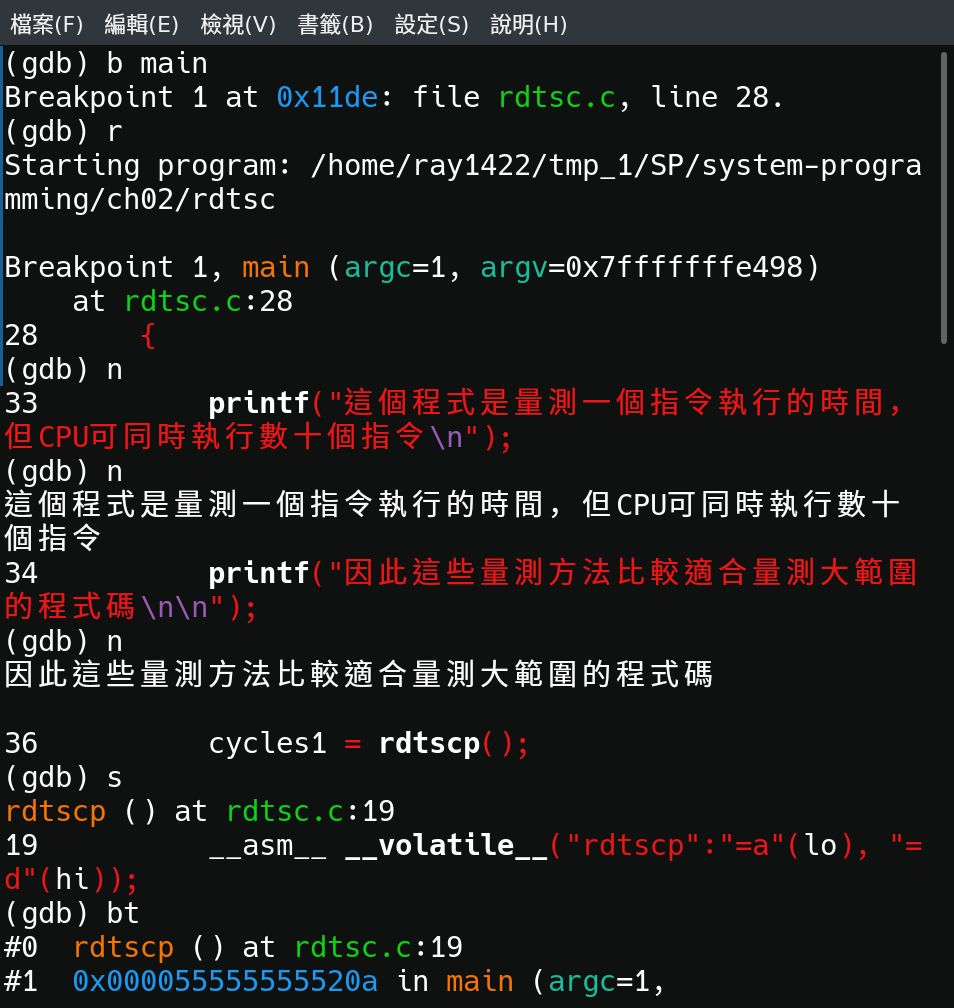
\includegraphics[width=1\linewidth]{p1.jpg}
\caption{Debugging with GDB (1)}
\label{fig:gdb_1}
\end{minipage}
\begin{minipage}[t]{0.49\textwidth}
\centering
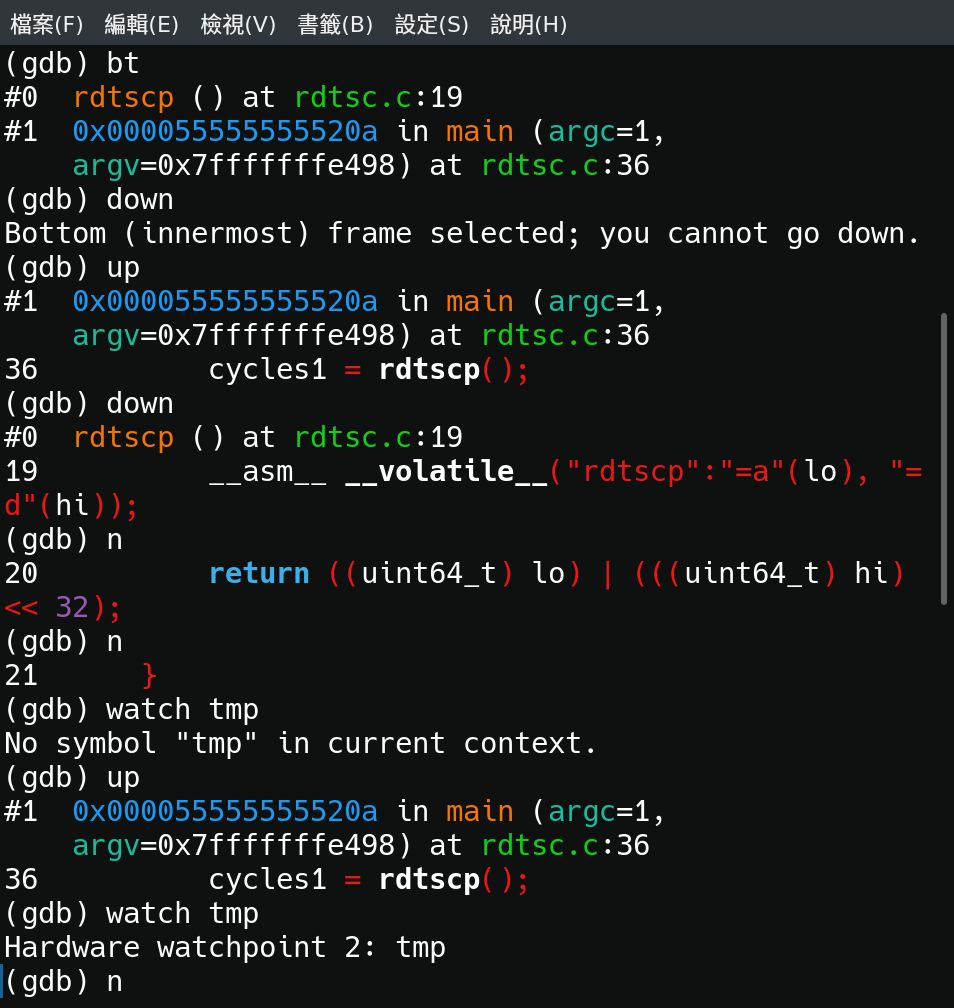
\includegraphics[width=1\linewidth]{p2.jpg}
\caption{Debugging with GDB (2)}
\label{fig:gdb_3}
\end{minipage}
\end{figure}
使用 \mintinline{bash}{gdb ./rdtsc} 開始除錯。\figurename\ref{fig:gdb_1} 使用 ``n'' 單步執行程式(不進入函數),使用 ``s'' 進入函數,使用``bt'' 檢視程式執行堆疊回朔。\figurename\ref{fig:gdb_2} 使用 ``up'' 及 ``down'' 移動目前聚焦的堆棧,使用 watch 追蹤變數值變更。

\subsection{除錯非法記憶體存取}
\begin{figure}[htbp]
    \centering
    \begin{minipage}[ht]{0.49\textwidth}
        \centering
        \begin{minted}{c}
        #include <stdio.h>
        int main() {
            int *a;
            *a = 10;
            printf("%d\n", *a);
        }
        \end{minted}
        \caption{非法記憶體存取的程式}
        \label{fig:c_vol_mem}
    \end{minipage}
    \begin{minipage}[ht]{0.49\textwidth}
        \centering
        \includegraphics[width=1\linewidth]{p4.jpg}
        \caption{Debugging with GDB (3)}
    \label{fig:gdb_2}
\end{minipage}
\end{figure}

如\figurename\ref{fig:c_vol_mem} 的程式,顯然 \mintinline{c}{a} 尚未初始化分配記憶體位址,賦值會造成非法記憶體存取。 \figurename\ref{fig:gdb_3} 中將斷點設在main並逐行執行,在賦值時發生錯誤並結束。


\end{document}
